\beginsong{Möge die Straße}[wuw={nach einem irischen Volkslied}, kssiv={326}, biest={611}, siru={164}]

% \beginverse
% \[F]Möge die \[C]Straße \[Dm]uns zusammen \[Am]führen
% \[H&]und der Wind in \[F]deinem Rücken \[C]sein.
% \[F]Sanft falle \[C]Regen \[Dm]auf deine \[Am]Felder
% und \[H&]warm auf dein Ge\[C]sicht der Sonnen\[F]schein. \[F7]
% \endverse

\beginverse
\endverse
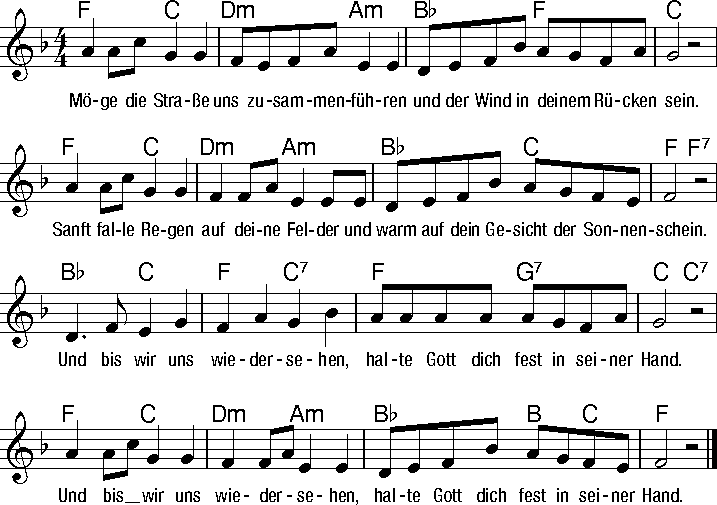
\includegraphics[page=1]{Noten/Lied115.pdf}

\beginverse\memorize
\[F]Führe die \[C]Straße, \[Dm]die du \[Am]gehest,
\[B&]immer nur zu \[F]deinem Ziel berg\[C]ab;
\[F]Hab, wenn es \[C]kühl wird \[Dm]warme Ge\[Am]danken 
\[B&]und den vollen \[C]Mond in dunkler \[F]Nacht. \[F7]
\endverse

\beginchorus
\[B&]Und bis \[C]wir uns \[F]wieder\[C7]sehen
\[F]halte Gott dich \[G7]fest in seiner \[C]Hand. \[C7]
\[F]Und bis \[C]wir uns \[Dm]wieder\[Am]sehen
\[B&]halte Gott dich \[C]fest in seiner \[F]Hand.
\endchorus

\beginverse
^Hab' unterm ^Kopf ein ^weiches ^Kissen,
^habe Kleidung ^und das täglich ^Brot;
^Sei über ^vierzig ^Jahre im ^Himmel,
be^vor der Teufel ^merkt: Du bist schon ^tot. ^
\endverse

\printchorus

\beginverse
^Bis wir ^uns mal ^wieder^sehen,
^hoffe ich, dass ^Gott dich nicht ver^lässt;
^Er halte ^dich in ^seinen ^Händen,
^drücke seine ^Faust dich nicht zu ^fest.
\endverse

\printchorus

\endsong
